\documentclass[10pt,journal,compsoc]{IEEEtran}

\usepackage[ngerman]{babel}
\usepackage[utf8]{inputenc}
\usepackage[T1]{fontenc}
\usepackage{graphicx}
\usepackage{listings}
\usepackage[svgnames]{xcolor} % Specify colors by their 'svgnames', for a full list of all colors available see here: http://www.latextemplates.com/svgnames-colors
\usepackage[font=small,labelfont=bf]{caption} % Required for specifying captions to tables and figures

\graphicspath{{images/}}

% correct bad hyphenation here
\hyphenation{}

\begin{document}
  \title{Railway-Oriented-Programming in Clojure -- \LARGE Funktionales Error-Handling}
  \author{Jan-Philipp~Willem,~Fakultät für Informatik, Hochschule Mannheim}
  \markboth{Railway-Oriented-Programming in Clojure -- Funktionales Error-Handling}{}

  \IEEEtitleabstractindextext{%
    \begin{abstract}
Das Verhalten eines Programms nach einem Fehlerfall zu definieren, wurde bereits in vielen Programmiersprachen zu lösen versucht.
In der Praxis wird oft nur an den “Happy-Path” gedacht, oder gar gescheut den Code durch eine komplizierte Fehlerbehandlung aufzublähen.
Scott Wlaschin hat versucht den Either-Type (Monade) mithilfe des Konzepts von einzelnen Abschnitten einer Eisenbahnstrecke auf eine andere Art zu erklären und damit eine funktionale Fehler-Beachtende Herangehensweise vorgeschlagen.
Im Folgenden soll eine Umsetzung dieser Ideen in der Sprache Clojure und dessen Möglichkeiten beschrieben werden.
    % \\
    % ~\\
    % \textbf{Abstract}---
    \end{abstract}
  }
  \maketitle

  \IEEEraisesectionheading{
    \section{Einleitung}\label{sec:einleitung}
  }
  \begin{center}
    \vspace{-1cm}
    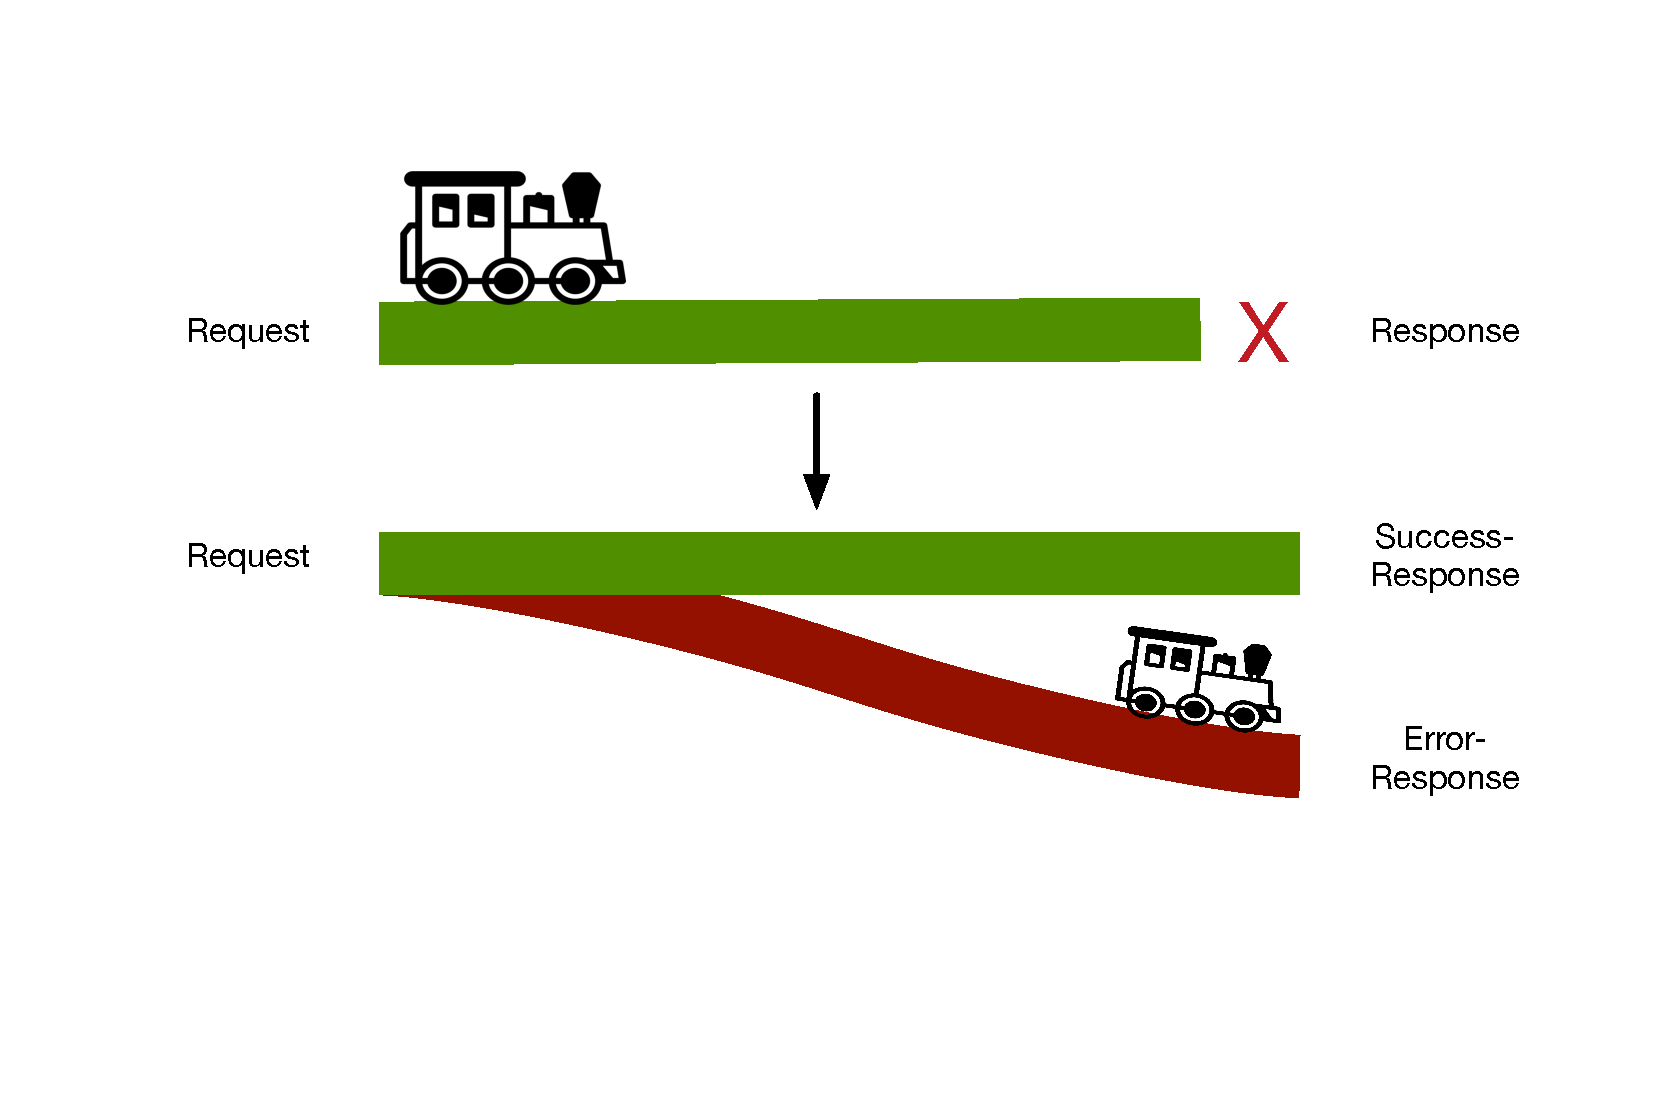
\includegraphics[width=.5\textwidth]{intro_rails_full.pdf}
    \vspace{-2cm}
    \captionof{figure}{Bisherige Fehlerbehandlung und Nutzen von Zwei-Wege-Schienenteilen}
  \end{center}
  \vspace{.6cm}

  \IEEEPARstart{S}{eit} es losging.
  \subsection{"`Happy-path"'}
  \subsection{"`Error-by-design"'}

  \section{Railway-Oriented-Programming}
  Es sollen zunächst folgende grundlegende Schienen-Teile betrachtet werden:
  \begin{itemize}
    \item Result: Success/Failure
    \item switch
    \item switch-functions
    \item bind/bind-pipe
    \item switch-compose
  \end{itemize}
  Die Grundüberlegung besteht in der Erwartung, dass eine Funktion von nun an nicht nur einen einzigen Rückgabewert besitzt.
  Es soll zwischen einem gutartigen Ergebnis (\textbf{Success}) und dem Fehlerfall (\textbf{Failure}) unterschieden werden können.
  Dies ist durch ein Leichtes erzielbar, indem man einen \textbf{Result}-Typ definiert, welcher das eigentliche Ergebnis einer Funktion oder eine Fehlermeldung enthält.\\
  Eine Funktion die unseren Result-Typ nutzt, soll im Weiteren als eine \textbf{switch-function} bezeichnet werden, da sie wie eine Weiche in der Bahnfahrt reagiert, welche den Datenfluss von dem Success-Path auf den Failure-Path leitet.\\
  Um eine bestehende Funktion in einen ROP-Datenfluss zu integrieren, kann sie mit \textbf{switch} vereint werden, womit ihr eigentliches Ergebnis in ein Success konvertiert wird.\\
  Um zwei switch-functions miteinander zu verbinden, wird die Funktion \textbf{bind} genutzt, welche die Success- und Failure-Paths miteinander verbindet.
  Da die Sprache Clojure ein Lisp ist, liegt es nahe, bind auch für die Übergabe einer Liste mit mehreren switch-functions zu definieren. So führt \textbf{bind-pipe} (>>=) die übergebenen Forms nacheinander aus und leitet jeweils das Ergebnis der nächsten Funktion als Parameter zu.
  Es entsteht ein in sich geschlossenes Zwei-Wege-Schienensystem.
  Dabei fühlt sich die Vorgehensweise an, als ob man das thread-first macro (->) genutzt hätte, welches man in anderen Sprachen auch als pipe oder left-to-right-composition bezeichnet.\\
  Mit \textbf{switch-compose} kann man switch-functions im Vergleich zu bind auf eine andere Art miteinander verbinden.
  Es kann so aus jeweils zwei switch-functions eine Komposition gebildet werden, welche sich benutzen lässt, als wäre es eine einzige Funktion. Die Verschachtelungstiefe ist dabei beliebig groß zu wählen.
  Es sind beide Wege für jeweilig andere Use-Cases sinnvoll.
  \subsection{Weitere Schienenteile}
  In Erweiterung zu den Grundlegenden Schienenteilen sind weitere folgende denkbar:
  \begin{itemize}
    \item try/catch
    \item log
    \item tee
    \item map-parallel
    \item ..
  \end{itemize}

  \section{Fazit}
  Abschließend ist zu sagen, dass das Konzept der Fehlerbehandlung über einen Result-Typ und dessen dazugehörigen Hilfsfunktionen am Anfang im Vergleich zu dem bisherigen Weg sehr kompliziert wirkt.
  Weiterhin ist bei der Arbeit mit einem Team darauf zu achten, dass alle Entwickler neue Funktionen in den ROP-Datenfluss integrieren sollten.
  Bei einer konsistenten Anwendung, kann es im Gegenzug wirklich hilfreich sein, da man nun nicht mehr raten muss, ob eine Funktion bei einem Fehler nun nichts tut, Null oder bspw. einen negativen Wert zurückgibt.
  Man erhält so eine stabile und leicht wartbare Basis für eigene Implementierungen.
  Es kann bspw. bei einer Formular-Validierung für ein Feld oder eine Überprüfung jeweilig ein Schritt in unserem ROP-Datenfluss dargestellt werden.\\
  Als ein gutes Beispiel sind die Grund-Funktionen von Elm \cite{elm} zu betrachten, welche grundsätzlich alle bei kritischen Stellen eine Result- oder Maybe-Monade für den Rückgabewert nutzen.\\
  Gegen Ende des Projektes wurde der Schreiber dieser Arbeit auf zwei weitere interessante Umsetzungen von ROP in Clojure aufmerksam. \cite{otherrop} bedient sich einer Clojure-Library \cite{clojurecats} welche Konzepte der Kategorie-Theorie umsetzt. Und eine weitere \cite{otherrop2}, welche bereits als Paket in Leiningen verfügbar ist.

  \begin{thebibliography}{1}
    \bibitem{clojurebook}
    D. Higginbotham, \emph{Clojure for the Brave and True},\\https://braveclojure.com
    \bibitem{railwayWlaschin}
      Scott Wlaschin, \emph{Railway-Oriented-Programming -- a functional approach to error handling}, https://fsharpforfunandprofit.com/rop/
    \bibitem{otherrop}
      ah45, \emph{railway oriented programming},\\https://gist.github.com/ah45/7518292c620679c460557a7038751d6d
    \bibitem{corematch}
      Clojure Core Team, \emph{Core.match -- a Pattern Matching Function}, https://github.com/clojure/core.match/wiki/Basic-usage
    \bibitem{otherrop2}
    HughPowell, \emph{railway-oriented-programming},\\
    https://github.com/HughPowell/railway-oriented-programming
    \bibitem{clojurecats}
      Funcool, \emph{Cats -- Category Theory and Algebraic abstractions in Clojure}, https://github.com/funcool/cats
    \bibitem{elm}
      Elm, \emph{Gut gelößtes Sprachkonzept mit Maybe \& Either in Elm}, https://guide.elm-lang.org/error\_handling
  \end{thebibliography}
  Die Links wurden zuletzt am 07.07.2017 besucht.
\end{document}
